\section{Marco Teórico}

\begin{frame}
\subsection{Internet de las Cosas}
\frametitle{Marco Teórico}
\framesubtitle{Internet de las Cosas}

La internet de las cosas es un sistema de dispositivos de computación interrelacionados, máquinas mecánicas y digitales, objetos, animales o personas que tienen identificadores únicos y la capacidad de transferir datos a través de una red, sin requerir de interacciones humano a humano o humano a computadora. \newline

\begin{itemize}
	\item Heroku
	\item Framework Laravel
	\item JSON
	\item Base de Datos
\end{itemize}

\end{frame}

\begin{frame}
\frametitle{Marco Teórico}
\framesubtitle{Internet de las Cosas}
\subsubsection{HTTP}
\begin{itemize}\item HTTP
	\begin{itemize}
		\item GET%: este método solicita una representación del recurso especificado. Las peticiones que lo usan, solo deben regresar datos.
		\item HEAD%: este método solicita una respuesta igual a una peticion GET, pero sin el cuerpo de la respuesta.
		\item POST%: se usa para enviar una entidad al recurso especificado, causando a menudo un cambio en el estado o efectos secundarios en el servidor.
		\item PUT%: reemplaza todas las representaciones actuales del recurso destino con la la petición de carga útil.
		\item DELETE%: esta petición elimina el recurso especificado.
		\item CONNECT%: establece un túnel para el servidor identificado por el recurso de destino.
		\item OPTIONS%: se usa para describir las opciones de la comunicación para el recurso destino.
		\item TRACE%: realiza una prueba de mensaje loop-back a lo largo de la ruta del recurso de destino. 
		\item PATCH%: se usa para realizar modificaciones parciales a un recurso.
	\end{itemize}
\end{itemize}

\end{frame}

\begin{frame}
\frametitle{Marco Teórico}
\framesubtitle{Smart House}

Smart House es un entorno que tiene sistemas sofisticados a través de los cuales se pueden controlar algunos de los objetos de la casa, como luces, puertas, ventanas, además puede racionalizar el consumo de energía, entre otras funciones mediante el uso de sensores. Básicamente, uno de los beneficios más importantes del uso de la tecnología en las casas, es la prestación de servicios a las personas.\cite{Howedi2016} 
\end{frame}

\subsection{Hardware}

\subsubsection{ESP-WROOM-32}

\begin{frame}
\frametitle{Marco Teórico}
\framesubtitle{ESP-WROOM-32}

Es un potente módulo MCU Wi-Fi + BT + BLE que se dirige a una amplia variedad de aplicaciones, desde redes de sensores de baja potencia hasta las tareas más exigentes, como codificación de voz, transmisión de música y decodificación de MP3, además de su reducido tamaño, según se observa en la figura \ref{fig:esp32-wroom-s32-00}.\cite{EW32}

\begin{figure}[H]
	\centering
	\caption{ESP WROOM 32. Tomado de: \cite{ESPIMG}\label{fig:esp32-wroom-s32-00}}
	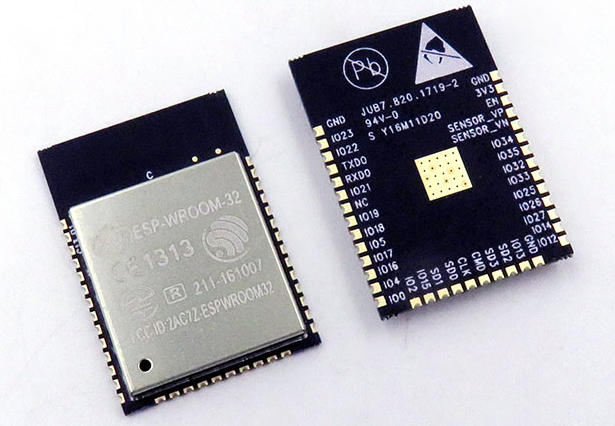
\includegraphics[width=0.4\linewidth]{Imagenes/esp32-wroom-s32-00}
\end{figure}
\end{frame}

\begin{frame}
\frametitle{Marco Teórico}
\subsubsection{Corriente Alterna (AC)}
{\small}
\textbf{Corriente Alterna (AC):}
``Es un tipo de corriente eléctrica, en la que la dirección del flujo de electrones va y viene a intervalos regulares o en ciclos. La corriente que fluye por las líneas eléctricas y la electricidad disponible normalmente en las casas procedente de los enchufes de la pared es corriente alterna. La corriente estándar utilizada en los EE.UU. es de 60 ciclos por segundo (es decir, una frecuencia de 60 Hz); en Europa y en la mayor parte del mundo es de 50 ciclos por segundo (es decir, una frecuencia de 50 Hz.)''. \cite{Cor}\newline

\subsubsection{Corriente Directa (DC):}
\textbf{Corriente Directa (DC)}
``Es la corriente eléctrica que fluye de forma constante en una dirección, como la que fluye en una linterna o en cualquier otro aparato con baterías es corriente continua.

Una de las ventajas de la corriente alterna es su relativamente económico cambio de voltaje. Además, la pérdida inevitable de energía al transportar la corriente a largas distancias es mucho menor que con la corriente continua''. \cite{Cor}
\end{frame}

\begin{frame}
\subsubsection{Control de potencia AC por ángulo de fase}
\frametitle{Marco Teórico}
\framesubtitle{Control de potencia AC por ángulo de fase}
\begin{wrapfigure}{r}{0.4\linewidth}
	\centering
	\caption{{\scriptsize Representación gráfica del ángulo de disparo y de conducción del TRIAC y de la carga. Tomado de: \cite{CEKIT}.}}
	\label{fig:triacgraph}
	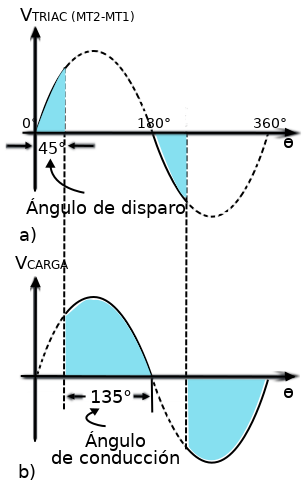
\includegraphics[width=0.6\linewidth]{Imagenes/TRIAC_graph}
\end{wrapfigure}
``Los SCR y los TRIAC, permiten aplicar una técnica muy conveniente y eficaz para controlar el voltaje promedio y por lo tanto la potencia aplicada a una carga, cambiando el ángulo de fase con el cual la fuente de voltaje se aplica a ésta. Esta técnica de control de voltaje es muy usada en las aplicaciones de regulación de motores, iluminación y temperatura, por ser el voltaje la variable principal en estos tres procesos''.\cite{CEKIT}

\end{frame}

\begin{frame}
\subsubsection{Control de Cargas DC}
\frametitle{Marco Teórico}
\framesubtitle{Control de Cargas DC}

\begin{wrapfigure}{r}{0.5\linewidth}
	\centering
	\caption{Ciclo Útil PWM. [Imagen Propia] }
	\label{fig:pwm-duty-800x396}
	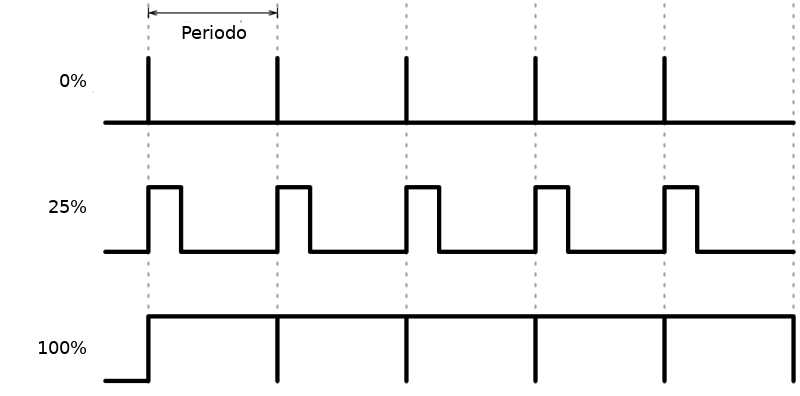
\includegraphics[width=0.9\linewidth]{Imagenes/pwm}
\end{wrapfigure}
Los transistores como switch permiten controlar las cargas de corriente continua con ayuda de una señal PWM que los activa o desactiva. Las cargas de corriente continuas típicas como los motores y LED's, a parte de poder funcionar en dos estados, encendido y apagado, pueden se controladas mediante la modulación por ancho de pulso (PWM), ya que al variar el ancho de pulso de la señal eléctrica se varia la cantidad de energía entregada a la carga, por ejemplo, si es un LED el cambio se refleja en su intensidad lumínica y si es un motor DC cambia su velocidad de giro \cite{PWM}.

\end{frame}

\subsubsection{Sensores}
\begin{frame}
\frametitle{Marco Teórico}
\framesubtitle{Sensores}

\begin{multicols}{3}
	
	\begin{figure}[!]
			\centering
			\caption{\tiny Modulo GY-30. Tomado de: \cite{GY30}}
			\label{fig:gy-30}
			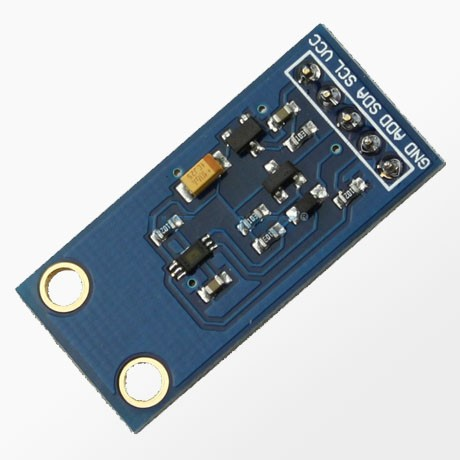
\includegraphics[width=0.4\linewidth]{Imagenes/gy-30}
	\end{figure}
	
	\begin{figure}[!]
		\centering
		\caption{\tiny Sensor DHT11. Tomado de: \cite{DHT11}}
		\label{fig:dht11}
		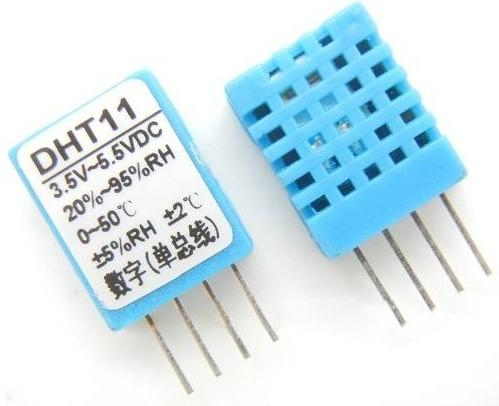
\includegraphics[width=0.4\linewidth]{Imagenes/dht11}
	\end{figure}
	
	
	\begin{figure}[!]
		\centering
		\caption{\tiny Sensor MQ-135. Tomado de: \cite{MQ1}}
		\label{fig:sensor-calidad-aire-mq135}
	 	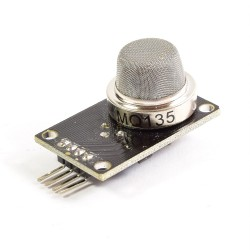
\includegraphics[width=0.3\linewidth]{Imagenes/sensor-calidad-aire-mq135}
	\end{figure}
	
	\begin{figure}[!]
		\centering
		\caption{\tiny Sensor de Lluvia. Tomado de: \cite{LLU}}
		\label{fig:yl-83}
		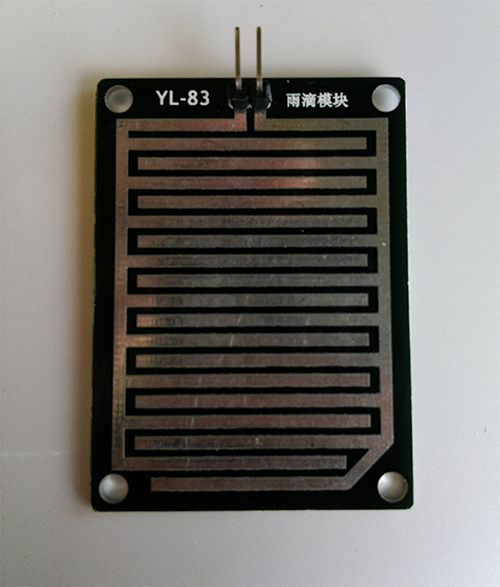
\includegraphics[width=0.35\linewidth]{Imagenes/YL-83}
	\end{figure}
	
	\begin{figure}[!]
		\centering
		\caption{\tiny Sensor HCSR501. Tomado de: \cite{PIR2}}
		\label{fig:sensor-hc-sr501-1000-m}
		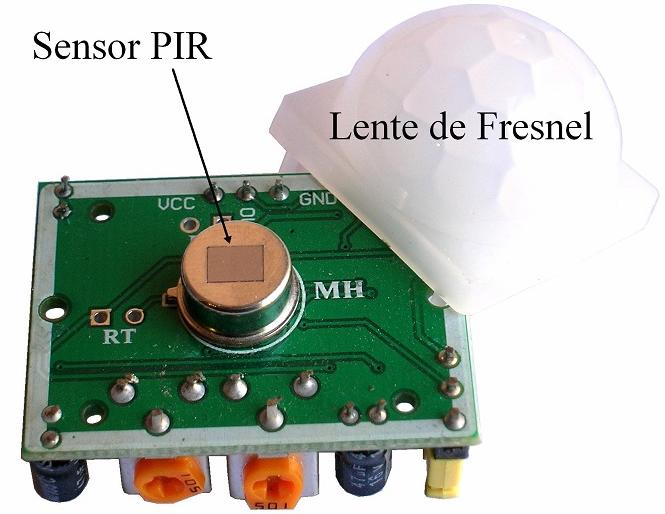
\includegraphics[width=0.5\linewidth]{Imagenes/SENSOR-HC-SR501-1000-M}
	\end{figure}
\end{multicols}

\end{frame}


\subsection{Software}
\begin{frame}
\frametitle{Marco Teórico}
\framesubtitle{Sistema Operativo en Tiempo Real}
\subsubsection{RTOS}

Los sistemas operativos en tiempo real, tienen como parámetro clave al tiempo, ya que en gran variedad de situaciones, por ejemplo, un proceso industrial, se requiere recolectar múltiples datos, los cuales son usados para el control de diversos procesos que deben ser ejecutados en determinados instantes, de no ser así, podría causar desde la mala ejecución de una tarea, hasta un accidente según la delicadeza del proceso.\newline

Los sistemas de computadoras de bolsillo y los sistemas integrados están diseñados para los consumidores, mientras que los sistemas en tiempo real son más adecuados para el uso industrial. Sin embargo, tienen ciertas características en común''. \cite{SO}
\end{frame}

\begin{frame}
\frametitle{Marco Teórico}
\framesubtitle{ESP-IDF}
\subsubsection{ESP-IDF}

ESP-IDF es el entorno de desarrollo oficial para el ESP32 desarrollado por Espressif System, el cual mediante una serie de comandos específicos escritos en la terminal (en el caso de linux), habilita la configuración del ESP32 en cuanto a su funcionamiento, es decir, permite encender o apagar características como el WiFi, el Bluetooth o realizar particiones de memoria, ademas de esto, se puede cargar el código por el puerto USB al ESP32, al igual que visualizar la información generada por el ESP32 por el mismo puerto. Este entorno se encuentra construido con diferentes características y APIs. \cite{ES}

\end{frame}